% This is a template to create your midterm report as a pdf.
% Just fill in the areas and run pdflatex
% For more information on LaTeX documents consult The (Not So
% Short Introduction to LateX2e
%
% to compile your report use the command
% pdflatex reportdocument.tex
%
% if you have \ref useage or other cross links
% you will have to run the above command again

% set 12pt font
\documentclass[12pt]{article}
% some useful packages
\usepackage[pdftex]{graphicx,color}
\usepackage{lscape}
\usepackage{hyperref}
\usepackage{fullpage}
\def\baselinestretch{1.5} % line spaceing
% set title
\title{Final Design Report \\
ECE437: Computer Design and Prototyping}
% fill in the blanks
\author{Jevin Sweval \\
        TA: Abhisek Pan}
% \today will put todays date
% or you can manually put the date in
\date{2010-04-30}
% cover page is a page by itself

\begin{document}
  \maketitle
  \newpage

% executive overview remember
% this should be on a page by itself
\section{Executive Overview}
As part of the ECE437 course, I have realized a MIPS-subset CPU in single-cycle, pipelined, pipelined with cache, and dual-core pipelined with cache forms that are synthesizable for the Cyclone II FPGAs. The subset of MIPS implemented allows for general purpose computing while still keeping the design simple. The first design completed, the single-cycle implementation, introduced me to the major components of the CPU: memory, ALU, control logic, and the register file. The single-cycle CPU works correctly for all test cases, runs at 22~MHz, and has an average CPI of $\approx 1.2$. The pipelined design required careful navigation of tricky data hazards (some of which were only unearthed during the last lab!) but paid off with a much faster clock rate. It runs correctly at 75~MHz with a CPI of $\approx 39$ with maximum memory latency. Instruction and data caches were added to the pipelined design in order to decrease the average memory access time. The caches slowed the design down to 28~MHz but drastically decreases the CPI to $\approx 6.1$ at maximum memory latency.\\

Using the cached, pipelined design, I created a dual core version of the CPU. This required a coherency controller between the data caches and an implementation of the MSI coherency protocol. In addition, the \texttt{LL}/\texttt{SC} instruction were implemented for locking. For the simple dual core design, I opted to include most of the coherency logic in the data caches themselves, making the coherency controller fairly trivial. This design decision would not scale to more cores but won in its simplicity for my purposes. The dual core design worked correctly for all test cases and ran at a glacial 7~MHz (due to long critical paths in the caches and a nearly full FPGA) with the same CPI slightly higher (due to memory access contention between cores) than the cached pipelined design. Of course, with two cores, the throughput is essentially doubled for embarrassingly parallel workloads. The dual core design was difficult to implement but I am now confident in my understanding of CPU design.\\

\newpage
\section{Processor and Cache Design}

All of the designs that I implemented closely followed the course textbook's designs. I feel that the most significant design choice was my coding methodology. All designs are coded almost entirely in behavioral VHDL. I find this type of code to be much easier to write and debug because it can be single-stepped in a debugger yet, if written carefully, can compile down to logic that is just as efficient as a structural design (excepting one case that I will talk about later). Also central to my coding methodology were VHDL records. The input and output signals to a block were wrapped in a record (similar to C \texttt{struct}s). Using records, one can add and remove signals to blocks without the time-consuming and error-prone edits of port and entity declarations. The records also group the signals in the waveform viewer, allowing for a tidier waveform window. I extensively use \texttt{numeric\_std} types and operators in my code to vastly cut down on code size (my ALU was two lines of code per operation) and to let the synthesizer automatically chose the best implementation in hardware. Most non-numeric types are declared as enumeration types. For example, the instructions are decoded into opcode enumerations. These enumerated types are human-readable in waveforms and source code instead of appearing as indecipherable bitstrings.\\

The pipelined design without cache was by far the fastest design in terms of clock speed. This is because the pipeline registers chopped up the critical path into much smaller parts. However, without a cache the performance was terrible with maximum memory latency (CPI $\approx 39$). Adding a 16-instruction instruction cache and a 64-word, 2-way associative, LRU data cache to the design reduced the CPI to $\approx 6.1$. The cost of this massive improvement to the CPI was a slower $f_{max}$. The cached design runs at 28~MHz but is about $2 \times$ as fast as the non-cached design in terms of wall time. This slowdown in clock speed was due to a very long critical path through the data cache. Examining the resulting FPGA resources indicated that the behavioral coding style utilized in the data cache created many unneeded, bloated muxes --- some over 1000 bits wide! I contemplated a redesign in pure RTL but the effort would have been too great.\\

The dual core design required more than simply copy-pasting two cores into a single VHDL file. I had to add a memory arbiter to arbitrate the RAM between the instruction caches and the coherency controller. This arbiter made sure to store the last serviced consumer so that no single consumer would be starved of data. The coherency controller sat between the two data caches and the memory arbiter Its purpose was to ensure data coherency thorough the MSI protocol. My implemented coherency controller was really just another memory arbiter that negotiated access to the RAM between the data caches, taking into account that one cache may need to perform a flush action on behalf of another. The majority of the coherency logic was placed into the data caches for simplicity. Each cache snoops the other cache's memory accesses. If both caches try to access the same line, one cache will wait for the other (the cache granted memory access via the coherency controller) to complete its access before continuing. To ensure consistency after processor writes to a shared line, a cache will direct its sibling to pause while it flushes the line to memory. The paused cache will then resume and read the written-back value from RAM. Each core has an \texttt{LL}/\texttt{SC} link register that is wired to the other core. Each core checks the other's link register during these atomic operations to ensure that they execute correctly. The dual core design, with two bloated data caches used $\approx 90\%$ of the FPGA resources (6 hour synthesis!). The fitter, faced with little breathing room was unable to keep the clock rate up. Thus, the final design runs at 7~MHz. The CPI is slightly increased over the single core design due to memory access contention. Especially during start-up, both cores are trying to fill their instruction and data caches and will often wait for the other memory consumers to finish before proceeding.


\newpage

\begin{landscape}

\begin{figure}
	\begin{center}
		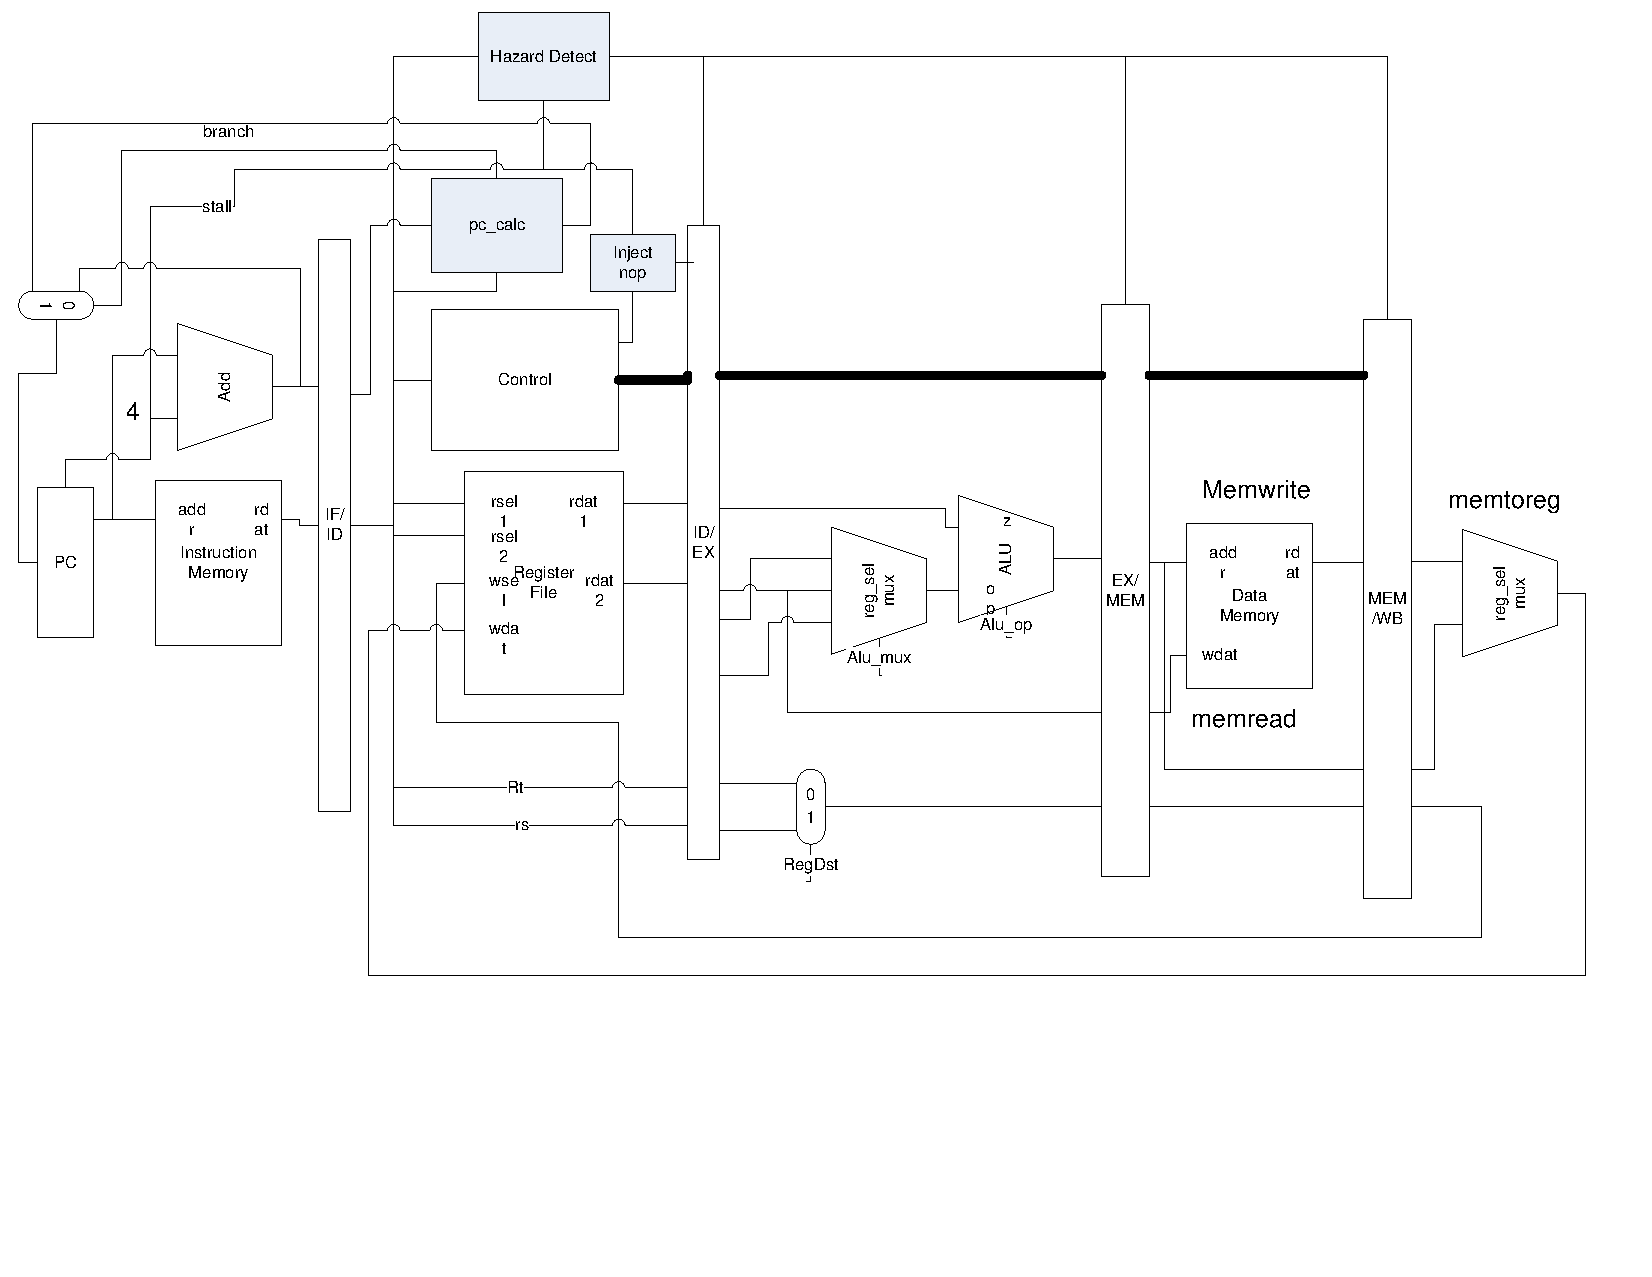
\includegraphics[width=7in]{bld_pipeline_branch}
	\end{center}
	\caption{Pipeline Block Diagram}
	\label{fig:pipeline}
\end{figure}

\end{landscape}

\newpage

\begin{figure}
	\begin{center}
		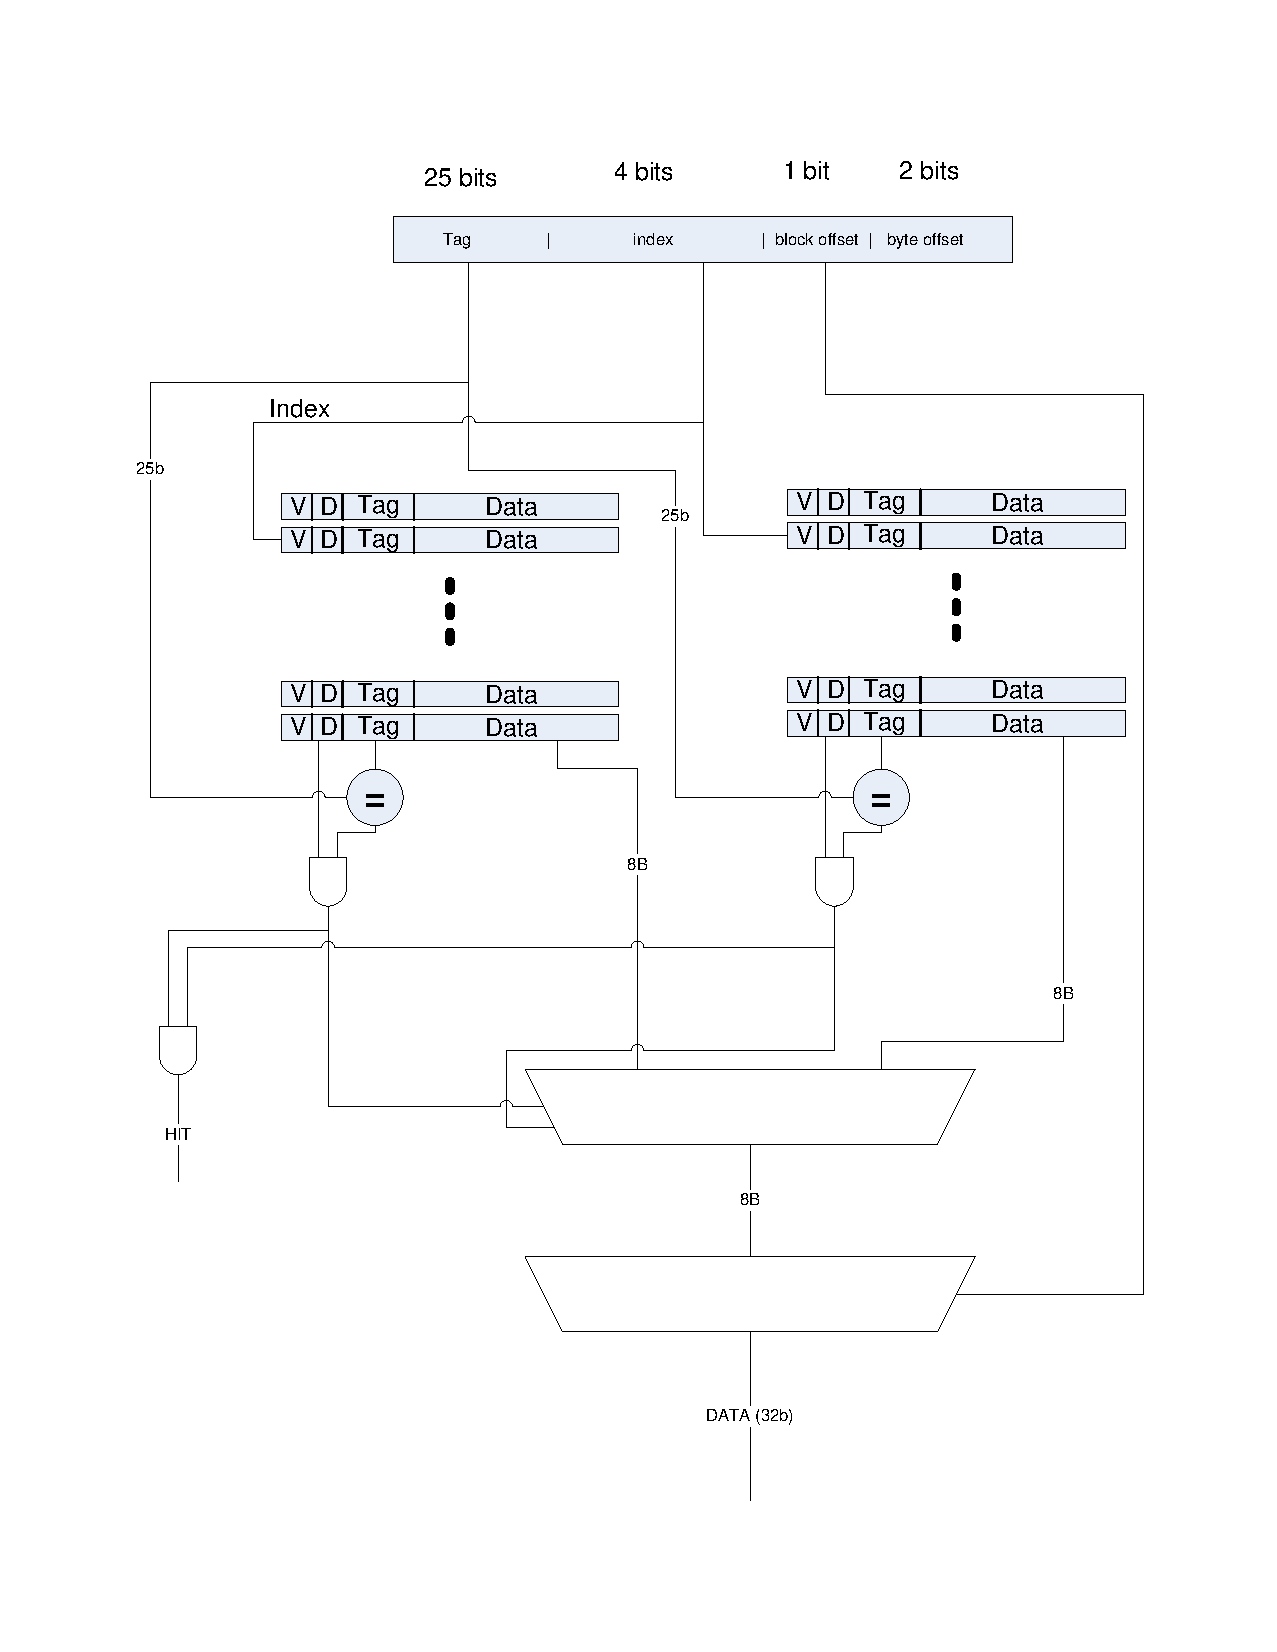
\includegraphics[width=7in]{dcache2}
	\end{center}
	\caption{Data Cache Block Diagram}
	\label{fig:dcache}
\end{figure}


\newpage

\begin{figure}
	\begin{center}
		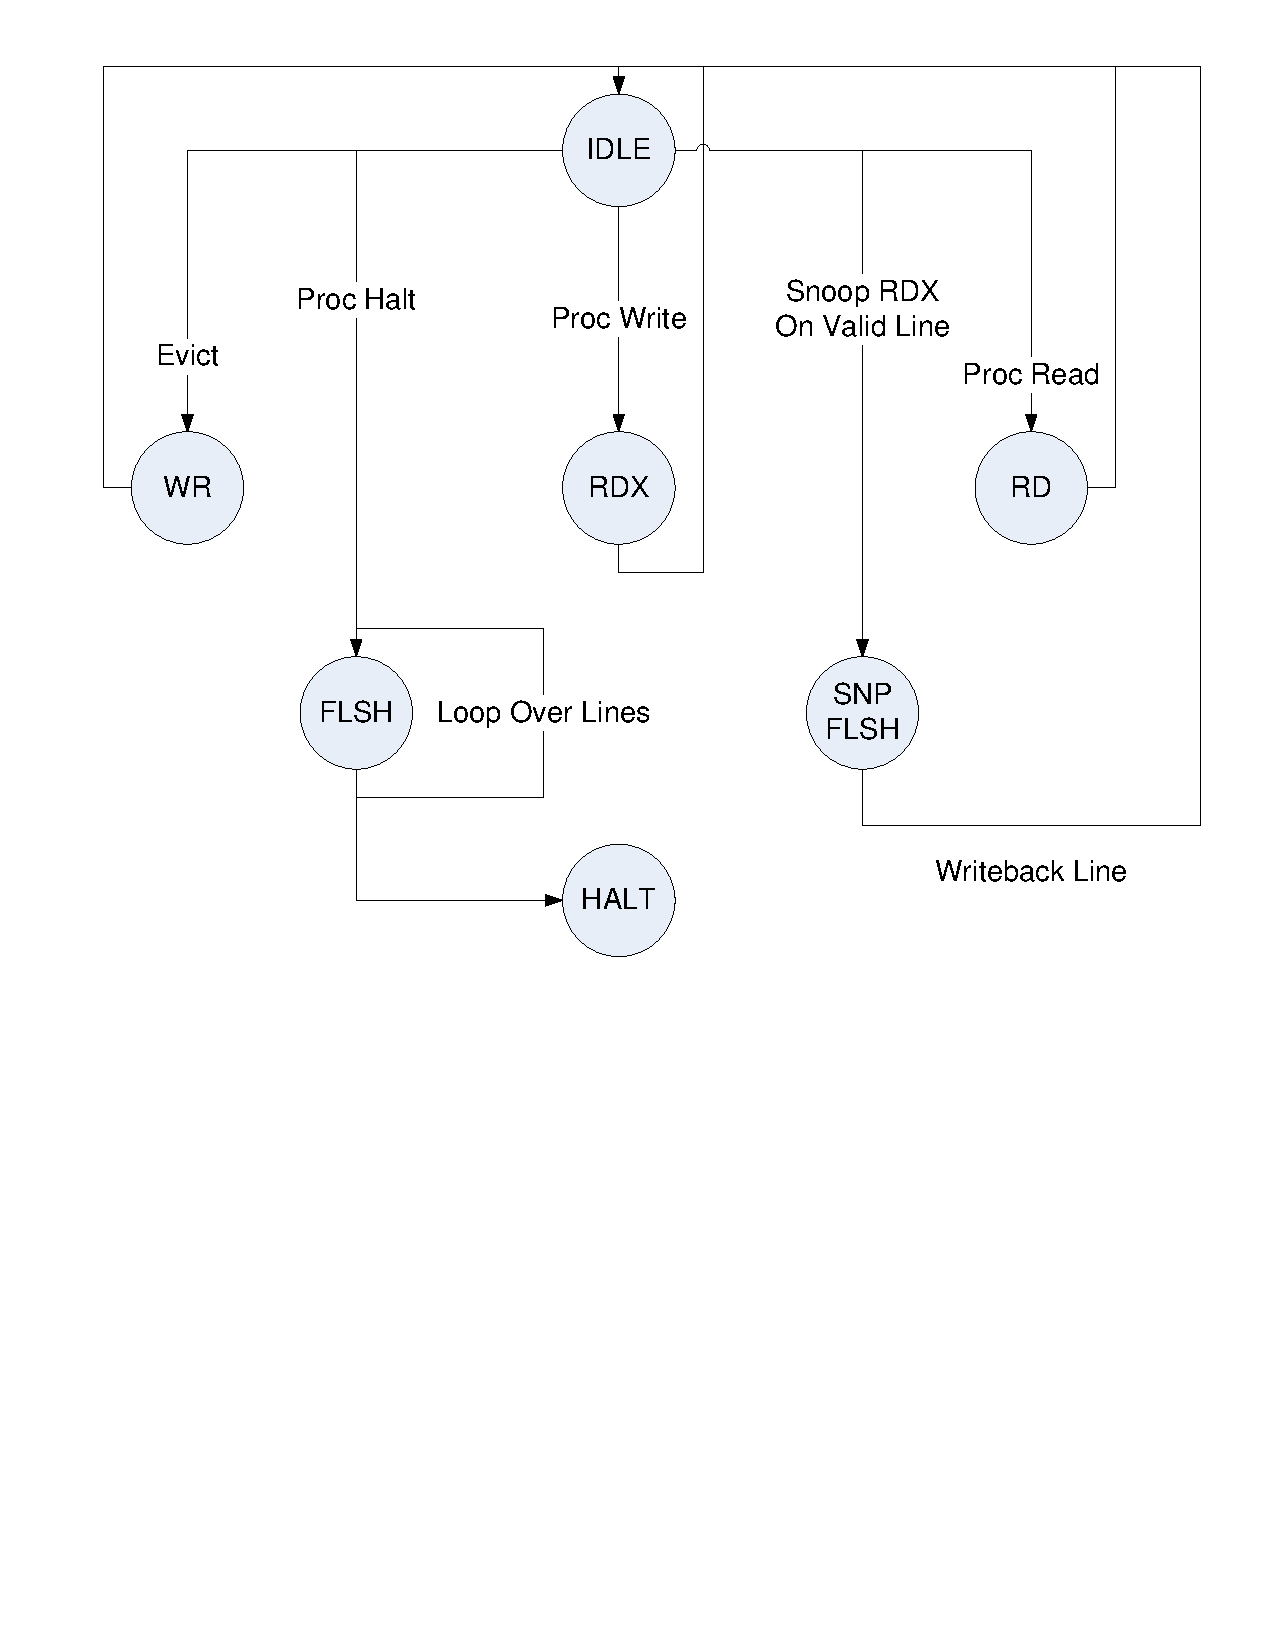
\includegraphics[width=7in]{cache_fsm}
	\end{center}
	\caption{Data Cache State Diagram}
	\label{fig:cache_fsm}
\end{figure}



\newpage

\begin{figure}
	\begin{center}
		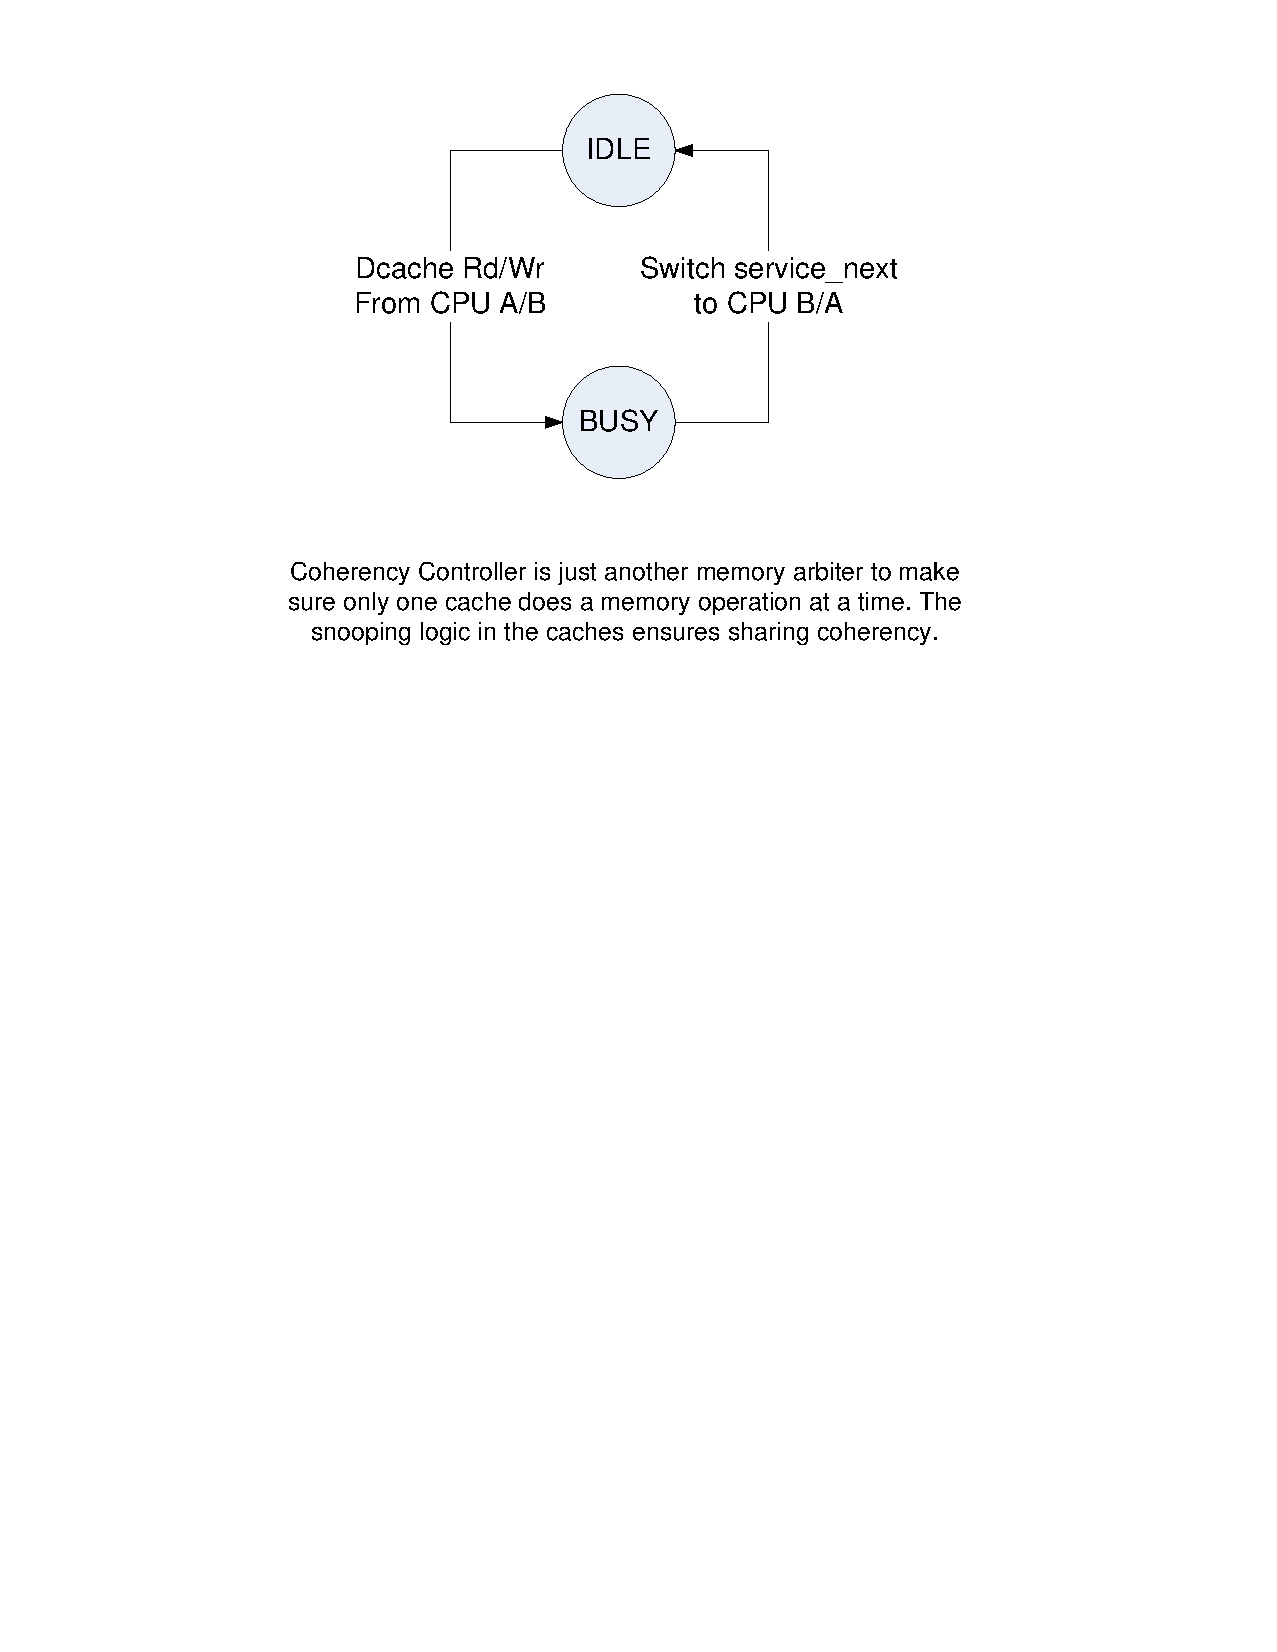
\includegraphics[width=7in]{cc_fsm}
	\end{center}
	\caption{Coherency Controller State Diagram}
	\label{fig:cc_fsm}
\end{figure}


\newpage

\begin{figure}
	\begin{center}
		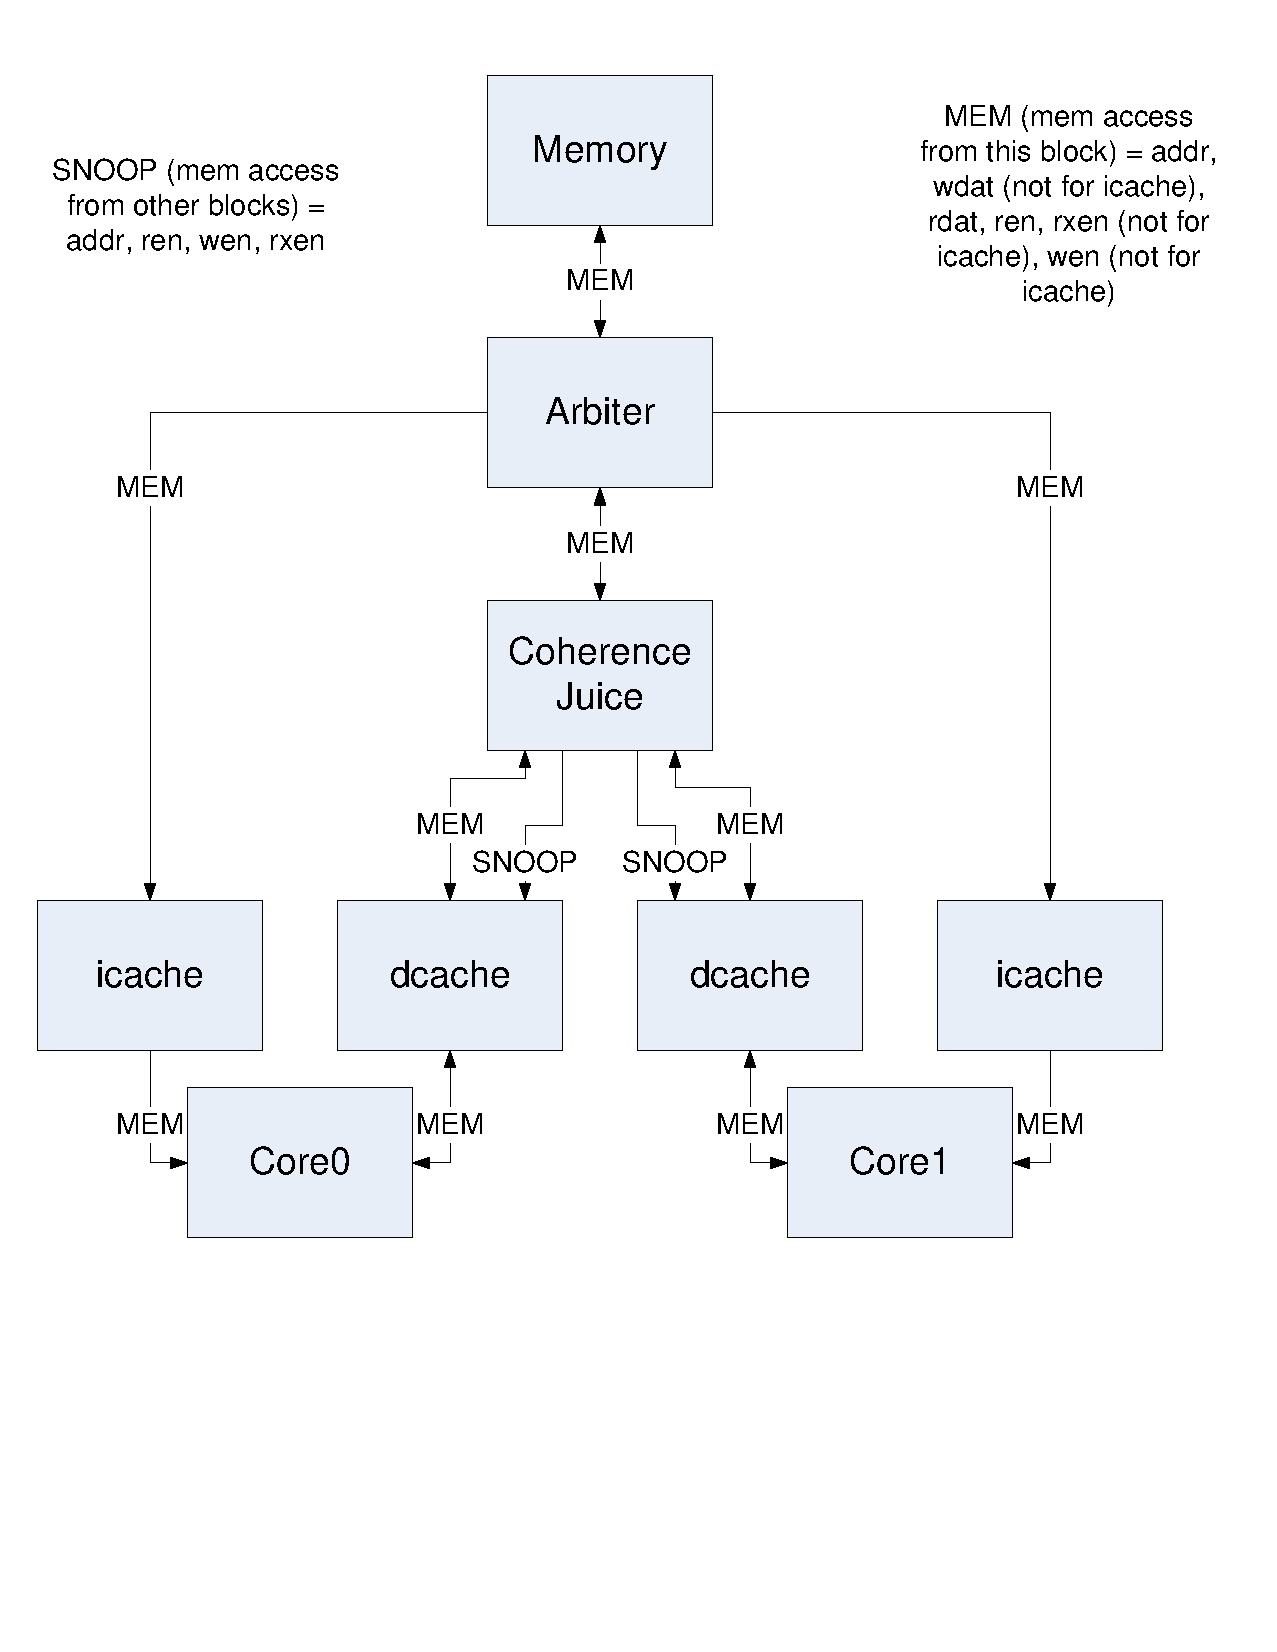
\includegraphics[width=7in]{multicore}
	\end{center}
	\caption{Multicore Block Diagram}
	\label{fig:dcache}
\end{figure}

\newpage

\newpage
\section{Processor Debug}

The output of the CPU is incorrect  because the \texttt{sw} instruction never actually wrote the value to memory.  The value \texttt{0x0000BEEF} should have been written to address \texttt{0x00000100}. One possible explanation for this behavior is a bug in the ID control logic. If the \texttt{sw} instruction was decoded incorrectly such that the \texttt{mem\_write} signal was not asserted, the instruction will never write to memory. The \texttt{mem\_write} signal originates from the control block in the ID stage and simply propagates through the pipeline registers until it reaches the MEM stage where it is consumed by the memory block. To find this bug, I would look at the \texttt{mem\_write} signal to ensure it is generated correctly by the control block and propigated by the pipeline registers correctly to the memory block.\\

Another possible explanation is that the controller which arbitrates access to the shared memory block is incorrect. If this is the case, even with a correct \texttt{mem\_write} signal, it is possible that the processor tries to perform a memory write operation while the \texttt{vram} block is not in the \texttt{ready} or \texttt{idle} state, resulting in no write. In this case, the problem originates at the memory arbiter and propagates when the arbiter fails to stall the pipeline until a \texttt{ready} or \texttt{idle} state. I could detect this by checking to make sure that \texttt{mem\_write} is only asserted when the \texttt{vram} is in the \texttt{ready} or \texttt{idle} state. The two bugs could be distinguished simply by viewing the waveforms and checking to see if either bug appears in the described portions of the waveforms. The bugs will not exhibit the same waveforms in the memory arbiter logic and control logic.\\

\newpage
  \section{Results}
  
The performance results for the design are displayed in Tables~\ref{tab:perf_single}--\ref{tab:perf_dual}. The single core design was the simplest implementation of the course's instruction set. The pipeline CPU added pipeline registers to break up the critical path, tripling the speed. The cached, pipelined design added instruction and data caches to the CPU to reduce the average memory access time. It performed excellently in doing so --- the CPI was reduced by $\approx 6.4 \times$.\\

\begin{table}
\begin{center}

  \caption{Single-cycle Performance (no memory latency)}
  \begin{tabular}{| c | c | c | c | c |}
  \hline
  f$_{\textrm{max}}$ (MHz) & CPI & Latency (ns) & LEs & Registers \\ \hline
 23 & 1.2 & 260 & 3,059 & 1,231 \\ \hline
  \end{tabular}
  \end{center}

  \label{tab:perf_single}
\end{table}

\begin{table}
\begin{center}

  \caption{Pipelined Processor Performance (max memory latency)}
  \begin{tabular}{| c | c | c | c | c |}
  \hline
  f$_{\textrm{max}}$ (MHz) & CPI & Latency (ns) & LEs & Registers \\ \hline
 75 & 39 & 2,600 &  3,045 & 1,475 \\ \hline
  \end{tabular}
  \end{center}

  \label{tab:perf_pipe}
\end{table}

\begin{table}
\begin{center}

  \caption{Cached, Pipelined Processor Performance (max memory latency)}
  \begin{tabular}{| c | c | c | c | c |}
  \hline
  f$_{\textrm{max}}$ (MHz) & CPI & Latency (ns) & LEs & Registers \\ \hline
 28 & 6.1 & 1,090 & 13,186 & 5,359 \\ \hline
  \end{tabular}
  \end{center}

  \label{tab:perf_cache}
\end{table}



\begin{table}
\begin{center}

  \caption{Dual Core, Cached, Pipelined Processor Performance (max memory latency)}
  \begin{tabular}{| c | c | c | c | c |}
  \hline
  f$_{\textrm{max}}$ (MHz) & CPI & Latency (ns) & LEs & Registers \\ \hline
 7 & 7.3 & 5,215 & 28,128 & 11,790 \\ \hline
  \end{tabular}
  \end{center}

  \label{tab:perf_dual}
\end{table}



  \section{Conclusion}

In this course I have designed a single-cycle and pipelined implementation of a MIPS-subset CPU. Both designs worked correctly and the pipelined design delivered a 57\% improvement in performance over the single-cycle design. The pipelined design necessarily had a higher CPI than the single-cycle design but the increase in f$_{\textrm{max}}$ more than compensated for this, improving the MIPS and latency over the simpler single-cycle design. The designs ran correctly up to clock rates slightly higher than the estimated f$_{\textrm{max}}$ returned by Quartus while exhibiting nondeterministic execution at any higher clock rates.\\

Through the course of the CPU designs, I learned first how a simple CPU is constructed, how its control logic is determined, and how a CPU design can be pipelined. The pipeline design gave me even more insight into debugging hardware designs that contain many signals and concurrent execution. By analyzing each design, I familiarized myself with how CPU performance is measured, how design choices affect performance, and how to compare the performance of designs in a meaningful manner. The single-cycle CPU has the advantage of being slightly simpler than the pipelined CPU to implement. However, the performance increase obtained by a straightforward pipelining is well worth the increase in design complexity. In terms of hardware resources used, both designs were essentially identical --- the pipelining was ``free'' in terms of resources. These CPUs could be used as an embedded processor in a System-on-a-Chip design. In this use, their performance is likely adequate as most of the heavy computations could be more quickly done in other IP-cores on the FPGA.\\

\end{document}
